
%(BEGIN_QUESTION)
% Copyright 2006, Tony R. Kuphaldt, released under the Creative Commons Attribution License (v 1.0)
% This means you may do almost anything with this work of mine, so long as you give me proper credit

Tegn utgangen for denne regulatoren med bare P-ledd, gitt et proporsjonalbånd på 125\%, bias lik 30\%, og omvendtvirkende reguleringsvirkning:

$$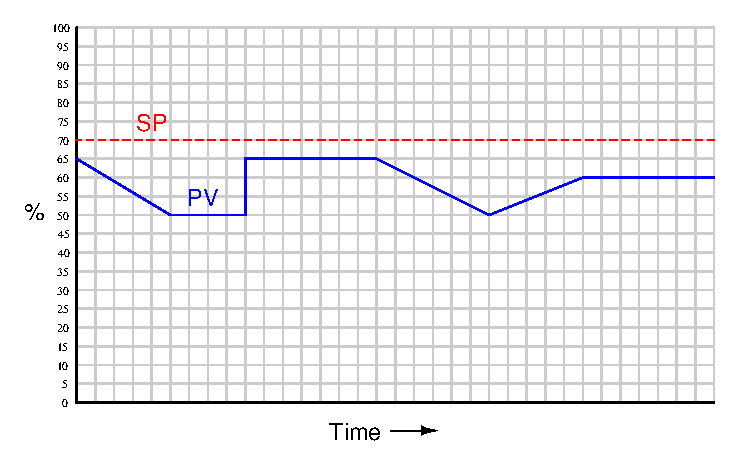
\includegraphics[width=15.5cm]{i01470x01.eps}$$

\vskip 20pt \vbox{\hrule \hbox{\strut \vrule{} {\bf Forslag til sokratisk diskusjon} \vrule} \hrule}

\begin{itemize}
\item{} Identifiser punkter på trenden der PV har positiv endringsrate.
\item{} Identifiser punkter på trenden der PV har negativ endringsrate.
\item{} Identifiser punkter på trenden der PV ikke endrer seg.
\item{} Hvordan ville utgangssignalets trend endres dersom {\it gain} i denne regulatoren ble økt?
\item{} Hvordan ville utgangssignalets trend endres dersom {\it bias} i denne regulatoren ble økt?
\item{} Hvordan ville utgangssignalets trend endres dersom regulatorens {\it virkemåte} ble byttet fra omvendt til direkte?
\end{itemize}

\underbar{file i01470}
%(END_QUESTION)





%(BEGIN_ANSWER)

$$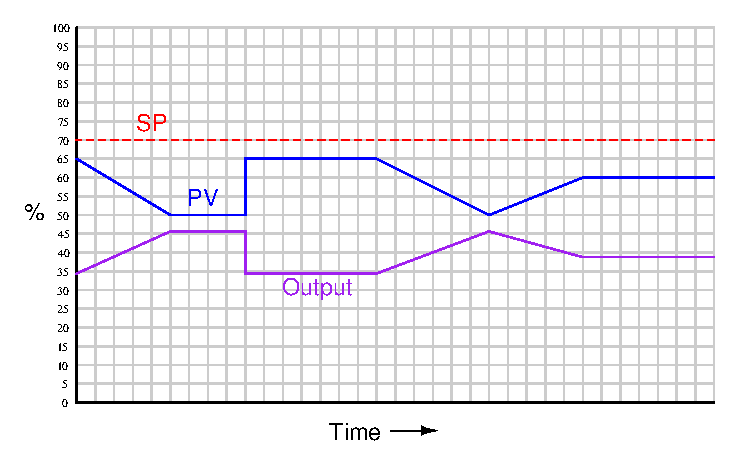
\includegraphics[width=15.5cm]{i01470x02.eps}$$

Med proporsjonalbåndverdi 125\% blir gain lik 0.8.

$$m = 0.8(\hbox{SP} - \hbox{PV}) + 30$$

% No blank lines allowed between lines of an \halign structure!
% I use comments (%) instead, so that TeX doesn't choke.

$$\vbox{\offinterlineskip
\halign{\strut
\vrule \quad\hfil # \ \hfil & 
\vrule \quad\hfil # \ \hfil & 
\vrule \quad\hfil # \ \hfil \vrule \cr
\noalign{\hrule}
%
% First row
{\bf PV} & {\bf SP} & {\bf Utgang} \cr
%
\noalign{\hrule}
%
% Another row
65\% & 70\% & 34\% \cr
%
\noalign{\hrule}
%
% Another row
50\% & 70\% & 46\% \cr
%
\noalign{\hrule}
%
% Another row
60\% & 70\% & 38\% \cr
%
\noalign{\hrule}
} % End of \halign 
}$$ % End of \vbox


%(END_ANSWER)





%(BEGIN_NOTES)


%INDEX% Control, proportional: graphing controller response

%(END_NOTES)

